\documentclass[11pt,a4paper]{article}

\usepackage[T1]{fontenc}
\usepackage[utf8]{inputenc}
\usepackage[slovene]{babel}
\usepackage{lmodern}
\usepackage{microtype}
\usepackage{geometry}
\usepackage{amsmath,amssymb}
\usepackage{enumitem}
\usepackage{fancyhdr}
\usepackage{tikz}

\geometry{margin=1.8cm}
\setlength{\parindent}{0pt}
\setlength{\parskip}{0pt}
\setlist[enumerate]{leftmargin=*,itemsep=0pt,topsep=0pt,parsep=0pt}
\pagestyle{fancy}
\fancyhf{}
\lhead{\small Matematika}
\rhead{\small Rešitve: kombinatorika}
\cfoot{\thepage}

\newenvironment{taskbox}[1]{%
    \par\addvspace{8pt}%
    \noindent\textbf{\large #1}\par
}{\par\addvspace{4pt}}

\begin{document}

\begin{center}
    {\LARGE\textbf{Rešitve in točkovnik}}\\[3pt]
    {\large Preizkus znanja: Kombinatorika \qquad 40 točk}
\end{center}

\begin{taskbox}{1. \hfill 10 točk \quad (predvideno: 13 min)}
\begin{enumerate}[label=\alph*)]
    \item Medalje so različne, zato je vrstni red pomemben; tekmovalec pa ne
    more dobiti več medalj. Gre za variacije brez ponavljanja:
    \[
        V_{11}^3=11\cdot10\cdot9=\boxed{990}.
    \]
    (1 t: prepoznava variacij brez ponavljanja, 2 t: pravilen produkt,
    1 t: rezultat)
    \item Vsako od petih mest PIN-kode lahko zasede katerakoli od 10 števk.
    Ponavljanje je dovoljeno, zato je število kod:
    \[
        10^5=\boxed{100\,000}.
    \]
    (1 t: 10 možnosti na mesto, 2 t: upoštevanje vseh petih mest in
    ponavljanja, 1 t: upoštevanje možnosti začetne ničle, 1 t: zapis potence,
    1 t: rezultat)
\end{enumerate}
\end{taskbox}

\begin{taskbox}{2. \hfill 5 točk \quad (predvideno: 7 min)}
Kombinatorično drevo za sendvič meni:
\begin{center}
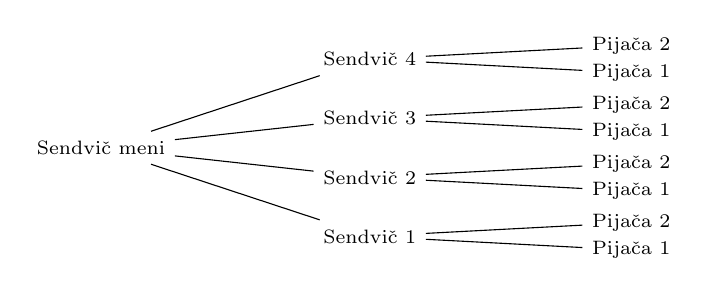
\begin{tikzpicture}[
grow=right,
level distance=2.7cm,
level 1/.style={sibling distance=0.75cm},
level 2/.style={sibling distance=0.35cm},
every node/.style={font=\scriptsize,anchor=west},
edge from parent/.style={draw}
]
\node {Sendvič meni}
child {node {Sendvič 1}
    child {node {Pijača 1}}
    child {node {Pijača 2}}}
child {node {Sendvič 2}
    child {node {Pijača 1}}
    child {node {Pijača 2}}}
child {node {Sendvič 3}
    child {node {Pijača 1}}
    child {node {Pijača 2}}}
child {node {Sendvič 4}
    child {node {Pijača 1}}
    child {node {Pijača 2}}};
\end{tikzpicture}
\end{center}
Topli meni ponuja \(3\cdot2\cdot3=18\) možnosti, sendvič meni pa
\(4\cdot2=8\). Ker izbiramo topli meni \textbf{ali} sendvič meni,
uporabimo pravilo vsote:
\[
    3\cdot2\cdot3+4\cdot2=18+8=\boxed{26}.
\]
(2 t: pravilno kombinatorično drevo za sendvič meni, 1 t: število toplih
menijev in sendvič menijev, 1 t: uporaba pravila vsote, 1 t: rezultat)
\end{taskbox}

\begin{taskbox}{3. \hfill 7 točk \quad (predvideno: 11 min)}
\begin{enumerate}[label=\alph*)]
    \item Pet soglasnikov obravnavamo kot en blok. Skupaj z dvema
    samoglasnikoma lahko razporedimo 3 enote na \(3!\) načinov, soglasnike
    znotraj bloka pa na \(5!\) načinov:
    \[
        3!\cdot5!=6\cdot120=\boxed{720}.
    \]
    (1 t: združitev soglasnikov v blok, 1 t: razporeditev bloka in
    samoglasnikov ter soglasnikov znotraj bloka, 1 t: rezultat)
    \item Beseda \textsc{kaktus} ima 6 črk, pri čemer se K ponovi dvakrat.
    Če bi črki K razlikovali, bi bilo \(6!\) razporeditev; zamenjava enakih
    črk K pa ne ustvari novega niza, zato delimo z \(2!\):
    \[
        \frac{6!}{2!}=\frac{720}{2}=\boxed{360}.
    \]
    (1 t: \(6!\), 1 t: imenovalec \(2!\), 1 t: pravilna formula,
    1 t: rezultat)
\end{enumerate}
\end{taskbox}

\begin{taskbox}{4. \hfill 9 točk \quad (predvideno: 15 min)}
\begin{enumerate}[label=\alph*)]
    \item Koeficienti pri četrti potenci so \(1,4,6,4,1\):
    \[
        (2x+3)^4
        =(2x)^4+4(2x)^3\cdot3+6(2x)^2\cdot3^2
        +4(2x)\cdot3^3+3^4
        =\boxed{16x^4+96x^3+216x^2+216x+81}.
    \]
    (1 t: koeficienti, 1 t: pravilno zapisani členi razvoja, 1 t: potence
    členov, 1 t: pravilna vstavitev, 1 t: pravilen rezultat)
    \item Za tretji člen velja \(k+1=3\), zato je \(k=2\). V formuli
    \(T_{k+1}=\binom{n}{k}a^{n-k}b^k\) vstavimo \(n=8\), \(a=x\),
    \(b=-2\):
    \[
        T_3=\binom{8}{2}x^{8-2}(-2)^2
        =28\cdot x^6\cdot4
        =\boxed{112x^6}.
    \]
    (1 t: \(k=2\), 1 t: pravilna formula, 1 t: vstavljene vrednosti,
    1 t: rezultat)
\end{enumerate}
\end{taskbox}

\begin{taskbox}{5. \hfill 9 točk \quad (predvideno: 14 min)}
V skupini je 9 fantov in 7 deklet.
\begin{enumerate}[label=\alph*)]
    \item Vrstni red izbire ni pomemben. Izberemo 2 od 7 deklet in 3 od 9
    fantov iz navedene skupine:
    \[
        \binom{7}{2}\binom{9}{3}=21\cdot84=\boxed{1764}.
    \]
    (1 t: uporaba kombinacij, 1 t: pravilna postavitev, 1 t: vrednosti
    binomskih koeficientov, 1 t: zmnožek, 1 t: rezultat)
    \item Preštejemo vse štiričlanske skupine iz iste skupine in odštejemo
    tiste brez deklet (torej skupine štirih fantov):
    \[
        \binom{16}{4}-\binom{9}{4}
        =1820-126
        =\boxed{1694}.
    \]
    (1 t: uporaba komplementa, 1 t: \(\binom{16}{4}\), 1 t:
    \(\binom{9}{4}\), 1 t: odštevanje in rezultat)

    Drugi način: ločeno preštejemo skupine z 1, 2, 3 ali 4 dekleti:
    \[
        \binom{7}{1}\binom{9}{3}
        +\binom{7}{2}\binom{9}{2}
        +\binom{7}{3}\binom{9}{1}
        +\binom{7}{4}
        =588+756+315+35
        =\boxed{1694}.
    \]
    (1 t: pravilno zajeti primeri z 1, 2, 3 ali 4 dekleti, 1 t: pravilno
    zapisani produkti kombinacij, 1 t: seštevanje delnih rezultatov,
    1 t: rezultat. Za nalogo 5b se prizna največ 4 točke; točkovanja za
    različna načina se ne seštevata.)
\end{enumerate}
\end{taskbox}

\begin{center}
    \textbf{Skupaj: 40 točk \qquad Predvideni čas: 60 minut}
\end{center}

\end{document}
